\section{Einleitung}

\subsection{Definition: Smart Home} % TODO redo this section

Wörtlich übersetzt, bedeutet der englische Begriff Smart Home so viel wie \textit{intelligentes Zuhause}. Intelligent meint hierbei die digitale und automatische Steuerung der Haustechnik.

Im Allgemeinen steht Smart Home dafür, für eine intelligente Vernetzung von elektrischen Verbrauchern in privaten Haushalten mit dem Ziel, den Wohnkomfort, die Sicherheit und die Energieeffizienz des Gebäudes zu steigern.\myfootcite[Vgl.][]{definition_smart_home}

Durch die Smart Home Technologie werden einerseits Alltagsvorgänge automatisiert, andererseits können die Geräte-Einstellungen, z.B. von Heizung, Licht und Lautsprechern, per Computer oder Smartphone schnell an die persönlichen Bedürfnisse angepasst werden ob zuhause oder unterwegs.

% is smart home only for private people or for business as well?

\begin{figure}[ht] % TODO this picture has nothing to do with smart home. it displays IOT!
	\centering
	\caption{Smart Home Mobiltelefonsteuerung}
	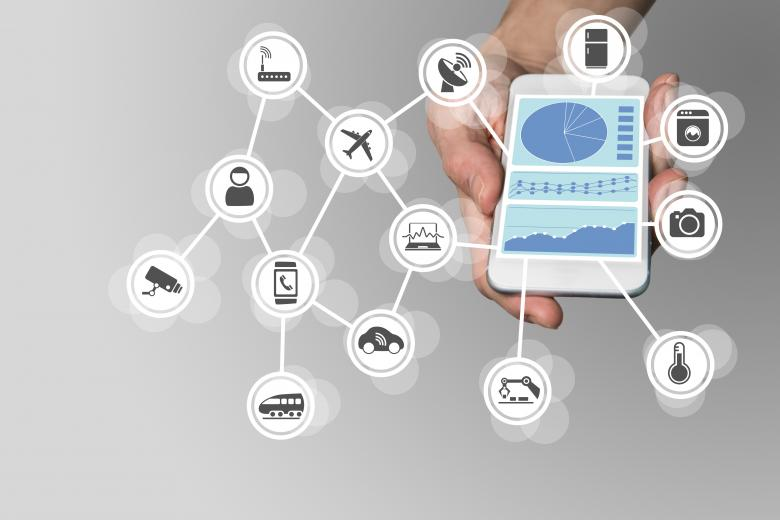
\includegraphics[width=0.8\textwidth]{smart_home_handy}
	\caption*{\footnotesize{Quelle: \mycite{figure_smart_home_handy}}}
	\label{fig:smarthomehandy}
\end{figure}

\subsection{Fragestellungen} % TODO better title

% folgende fragen ausformulieren:
% wie funktioniert ein smart home?
% wie kann man ein smart home system monetarisieren?

\section{Evaluation}

\subsection{Internet of Things}

Das \ac{IoT} hat zunächst nichts mit Heimautomatisierung zu tun.
Unter dem Internet der Dinge versteht man grundlegend die Verbindung von Geräten untereinander, sowie mit dem Internet.\myfootcite[Vgl.][]{ibm_iot}
Durch die Verbindung verschiedener Geräte, wie etwa einer Lichtschranke und einer Glühbirne, kann Mehrwert für den Benutzer der Geräte geschaffen werden, indem z.B. die Glühbirne automatisch bei Aktivierung der Lichtschranke aktiviert wird.
Zu einer Anwendung des \acp{IoT} wird das Beispiel, wenn das Internet noch mit involviert wird.
So wären hier Benachrichtigungen zu Bewegungsmeldungen oder Steuerung der Glühbirne über das Internet denkbar.

Ein Smart Home System kann also zum \ac{IoT}-System werden, wenn die Steuerung oder Automatisierung über eine Instanz im Internet abgewickelt wird.
Dies muss jedoch nicht der Fall sein.
So stellt die Software Home Assistant z.B. die Möglichkeit ein Smart Home System komplett offline zu betreiben.\myfootcite[Vgl.][]{hass_vision}

\subsection{Aufbau eines Smart Home Systems}

Aschendorf beschreibt den Aufbau von Smart Home Systemen als stufenförmige Hierarchie.
\autoref{fig:automatisierungspygramide} zeigt die drei Ebenen der Automatisierungspyramide nach Aschendorf:
Die \textit{Feldbusebene}, die \textit{Automatisierungsebene} und die \textit{Leitebene}. \myfootcite[Vgl.][59]{aschendorf14}

\begin{figure}[ht]
	\centering
	\caption{Automatisierungspyramide nach Aschendorf}
	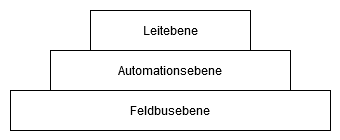
\includegraphics[scale=0.8]{Automatisierungspyramide_nach_Aschendorf}
	\caption*{\footnotesize{Quelle: Eigene Darstellung.}}
	\label{fig:automatisierungspygramide}
\end{figure}

\subsubsection{Feldbusebene}

Die Feldbusebene besteht aus sämtlichen eingebauten Systemkomponenten, also Gateways, welche verschiedene Systeme verbinden, Sensoren, welche z.B. Temperatur und Luftfeuchtigkeit überwachen, und Aktoren, wie z.B. Glühbirnen.
In der selben Ebene finden sich auch die Verbindungen der oben genannten Geräte wieder.
So ist die Feldbusebene in sich bereits funktional und direkt nutzbar.
Es kann z.B. der Sensor \textit{Lichtschalter 3} ausgelöst werden, welcher den Aktor \textit{Deckenlampe Wohnzimmer} aktiviert.\myfootcite[Vgl.][66-67]{aschendorf14}

\subsubsection{Automatisierungsebene}

Geräte übergreifende Automatisierungen werden in der Automatisierungsebene implementiert.
Dies wird durch einfache Controller oder programmierbare Mikrocomputer realisiert.
Nach der Änderung von Zuständen, wie z.B. der aktuellen Zeit, die Anwesenheit eines Bewohners oder die Temperatur eines Raumes, passt sich das Smart Home System mit dieser zusätzlichen Ebene nun nach vorgegebenen Regeln autonom an.\myfootcite[Vgl.][67-68]{aschendorf14}

\subsubsection{Leitebene}

Die Leitebene widmet sich der Interaktion des Smart Home Systems mit dessen Bewohnern.
Es lässt sich die Interaktion teilen in Eingaben und Ausgaben.
Zu den Eingaben zählen Befehle, die z.B. über Steuerungs-Apps gesendet werden oder von einem zentralen Steuerungscomputer emittiert werden.
Ausgaben werden etwa über digitale Dashboards auf diversen Displays angezeigt.
Über dieselben werden meist auch Fehlerdiagnosemeldungen angezeigt.\myfootcite[Vgl.][68-70]{aschendorf14}

% here we can use one of the required methods! (e.g. SSA)

\subsection{Kommunikationssysteme} % (auswahl)

% foreach:
% how does it work?
% use cases?
% pros and cons?

\subsubsection{LAN und WLAN}

% mention MQTT as a smart home / iot protocol

\subsubsection{ZigBee}
\subsubsection{Z-Wave}
\subsubsection{RFID}

\subsection{Amazon Alexa}

Amazon Alexa ist die Software für einen intelligenten Sprachassistenten, bestehend aus einem Lautsprecher, einem Mikrofon sowie einer Internetanbindung, welche seit 2014 in Alexa Geräten, wie in \autoref{fig:alexa_devices}, verbaut wird.\myfootcite[Vgl.][]{alexa_release}
Über die Internetanbindung wird auf ein Amazon Rechenzentrum zugegriffen, in welchem Ressourcen für die Verarbeitung von Spracheingaben mit \ac{ASR} und \ac{NLU} bereitgestellt werden.

\begin{figure}[ht]
	\centering
	\caption{Alexa Devices}
	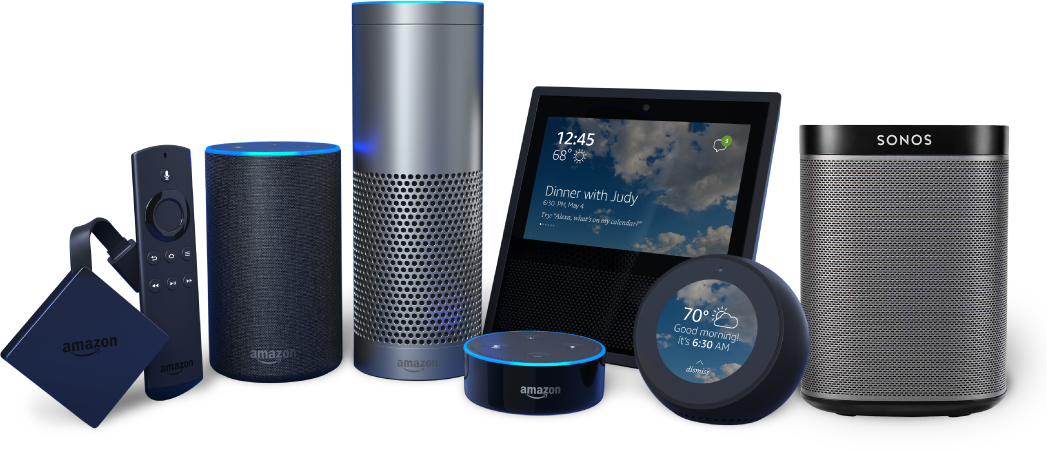
\includegraphics[scale=.8]{alexa_devices}
	\caption*{\footnotesize{Quelle: \mycite{figure_alexa_devices}}}
	\label{fig:alexa_devices}
\end{figure}

Unter \ac{ASR} versteht man die Umwandlung von menschlicher Sprache in Text.
Die Auslagerung der Rechenleistung in die Cloud sorgt für eine Beschleunigung der \ac{ASR}, sodass nahezu keine Latenz zu bemerken ist.\myfootcite[Vgl.][]{alexa_asr}

Lokal ist eine weitere \ac{ASR} Einheit verbaut, welche im Betrieb nach dem Stichwort \glqq Alexa\grqq \ lauscht.
Bei Erkennung des Stichworts werden nachfolgende Spracheingaben in Echtzeit an die Amazon Cloud gesendet.
Dort wird zunächst durch \ac{ASR} die Spracheingabe in Text konvertiert.
Anschließend wird durch \ac{NLU} über Mustererkennung die Bedeutung der Worte identifiziert. \myfootcite[Vgl.][]{alexa_nlu}

So können Befehle an ein Alexa Gerät weitergeben werden, welche über \ac{AWS}, Amazons Cloud, mit beliebigen Aktion verknüpft werden können.
Bspw. kann der Befehl \glqq Alexa, mach mir einen Kaffee.\grqq \ über \ac{AWS} mit der \ac{IoT}-Steuerung einer Kaffeemaschine so verknüpft werden, dass diese dann einen Kaffee produziert.
Die Verknüpfung von Befehl und Aktion über Alexa wird als \glqq Alexa Skill\grqq bezeichnet.
Zusätzlich gibt es \glqq Alexa Routines\grqq, welche keine Benutzereingaben entgegennehmen, also Automatisierungen darstellen können.

Mit Alexa Skills und Routines können Steuerungsebene, aber auch Automatisierungsebene eines Smart Home Systems realisiert werden.\myfootcite[Vgl.][]{alexa_skills_kit}

\begin{wrapfigure}{r}{0.35\textwidth}
	\centering
	\caption{Works with Alexa Siegel}
	
\includegraphics[scale=.5]{works-with-alexa}
	\caption*{\footnotesize{Quelle: \mycite{figure_works_with_alexa}}}
	\label{fig:works_with_alexa}
\end{wrapfigure}

Smart Home Produkte werden über das Internet mit Alexa verbunden.
Über Skills oder manuelle Programmierung kann ein Gerät, sofern es über ein öffentliches \ac{API} verfügt, angebunden werden.
Um diesen Prozess noch weiter zu vereinfachen können Hersteller die Zertifizierung \glqq Works with Alexa\grqq \ für ihre Produkte erlangen, wenn Spezifikationen bzgl. Installation des Produkts, sowie dessen Schnittstelle erfüllt werden.
\autoref{fig:works_with_alexa} zeigt das Works with Alexa Siegel, welches bei erfolgreicher Zertifizierung benutzt werden darf.
Für Besitzer von zertifizierten Geräten gibt es meist nur noch ein kurzen standardisierten Einrichtungsprozess zu überwinden.\myfootcite[Vgl.][]{workswithalexa}

% easy to use
% internet required
% data compromised
% closed source

% \begin{figure}[ht]
% 	\centering
% 	\caption{Amazon Alexa Voice Control}
% 	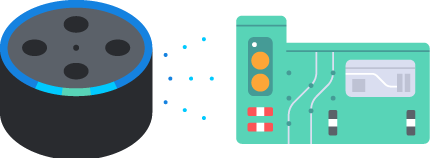
\includegraphics[scale=1]{echo_dot}
% 	\caption*{\footnotesize{Quelle: \mycite{figure_alexa_echo_dot}}}
% 	\label{fig:echo_dot}
% \end{figure}

\subsubsection{Vorteile}

% easy to use

\subsubsection{Nachteile}

% internet required
% data compromised
% closed source

\subsection{Home Assistant}

Home Assistant ist eine Open-Source-Software für Heimautomatisierung.
Durch den modularen Aufbau der Software können Entwickler einfach neue Smart Home Produkte implementieren.
So sind aktuell 1187 Smart Home Produkte über 46 Kategorien mit Home Assistant nutzbar.\myfootcite[Vgl.][]{hass_components}

\begin{figure}[ht]
	\centering
	\caption{Home Assistant Core Architektur}
	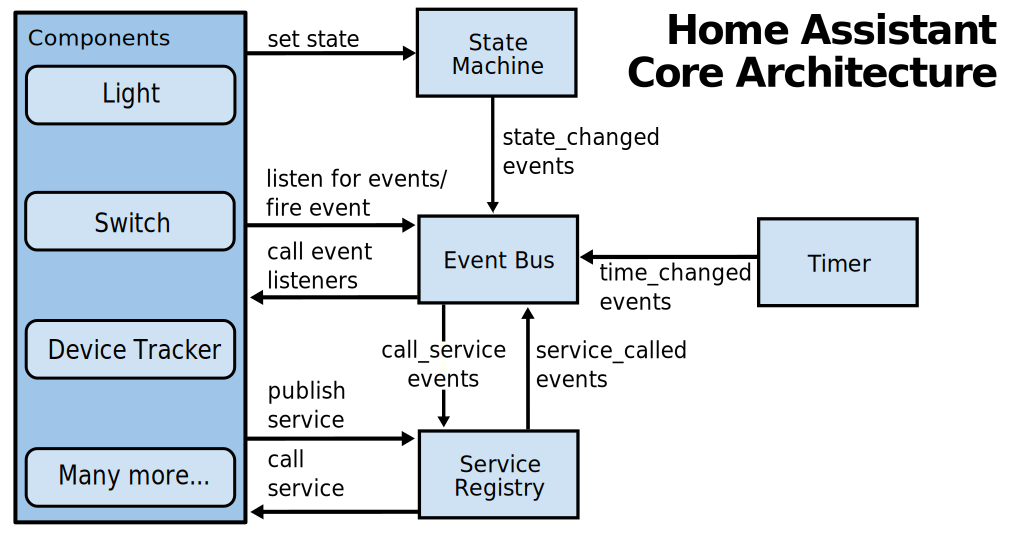
\includegraphics[width=0.9\textwidth]{hass_architecture}
	\caption*{\footnotesize{Quelle: \mycite{hass_architecture_figure}}}
	\label{fig:hasscorearch}
\end{figure}

\autoref{fig:hasscorearch} zeigt die Architektur, welche Home Assistant die Modularität verleiht.
Smart Home Produkte werden als Komponenten implementiert, welche mit dem Home Assistant Core interagieren.
Der Home Assistant Core besteht aus vier Modulen:

Das \textit{State Machine} Modul bildet den Status der verschiedenen Komponenten ab.
Bemerkt ein Fenstersensor z.B. dass ein Fenster geöffnet wurde, aktualisiert die Komponente \textit{Fenstersensor} ihren Status im \textit{State Machine} Modul, indem sie eine Nachricht an das Modul schickt.

Für zeitbasierende Automatisierungen existiert das Modul \textit{Timer}, welches sekündlich ein Event emittiert.
Ein Event ist eine Nachricht, welche beim Auftreten von definierten Bedingungen automatsich verschickt wird.

Über das \textit{Event Bus} Modul werden Events von den beiden bereits genannten Modulen empfangen von diesen ausgehend wiederum Events ausgelöst.

Das \textit{Service Registry} Modul bietet Komponenten die Möglichkeit beim Gesamtsystem einen Service zu registrieren.
Das Gesamtsystem wiederum kann über das selbe Modul den Service einer Komponente in Anspruch nehmen.
So kann eine Glühbirne z.B. den Service \textit{Glühbirne anschalten} registrieren, welcher dann von einer anderen Komponente, z.B. einem Lichtschalter, indirekt, über ein Event, aufgerufen werden kann.

Mit dieser Architektur kann eine neue Komponente implementiert werden, ohne dass der Home Assistant Core berührt wird.
Eine neue Komponente muss lediglich einen Service registrieren, auf ein Event reagieren oder ein Event auslösen können.\myfootcite[Vgl.][]{hass_architecture}
Die Implementierung einer neuen Komponente ist ausführlich in der Home Assistant Dokumentation beschrieben.\myfootcite[Vgl.][]{hass_implement_component}

Veröffentlicht wird Home Assistant unter der Apache 2.0 Lizenz.\myfootcite[Vgl.][]{hass_license}
Die Software ist also kommerziell und privat kostenlos nutzbar.
Lediglich die Marke \textit{Home Assistant} wird geschützt, sowie die Haftung und die Garantie ausgeschlossen.

Für die Weiterentwicklung von Home Assistant wurden im September 2018 vier Grundsätze definiert\myfootcite[Vgl.][]{hass_vision}:

\begin{itemize}
	\item Privatsphäre - alle Daten werden lokal verarbeitet und gespeichert.
	\item Lokale Kontrolle - es ist kein Internetanschluss notwendig.
	\item Offener Quelltext - die Funktionsweise kann jederzeit nachvollzogen werden.
	\item Interoperabilität - es soll einfach sein Apps mit Home Assistant zu verbinden
\end{itemize}

Ebenso wurde Nabu Casa Inc., als Modell für die Finanzierung der Entwicklung von Home Assistant, vorgestellt.
Home Assistant Nutzer können ihre private Instanz mit Nabu Casa um die Home Assistant Cloud Komponente für 5 USD pro Monat erweitern, was Home Assistant \ac{IoT}-Charakter verleiht.
Nabu Casa setzt dazu Software mit offenem Quelltext ein, verspricht keine Daten zu speichern und stellt dem Projekt Home Assistant Entwicklungkapazitäten zur Verfügung.\myfootcite[Vgl.][]{nabucasa}

\subsubsection{Vorteile}

Mit Home Assistant lassen sich hohe Kosten für zertifizierte Geräte sparen.
Während andere Smart Home System Anbieter, wie z.B. Amazon Alexa, Geräteherstellern die Implementierung von geeigneten Schnittstellen vorschreiben, damit die Geräte mit der jeweiligen Plattform genutzt werden können\myfootcite[Vgl.][]{workswithalexa}, bietet Home Assistant viele verschiedene Wege ein Geräte zu verbinden.
So sind über 1000 Schnittstellen bereits in Home Assistant implementiert\myfootcite[Vgl.][]{hass_components} und zusätzlich können neue oder eigen gebaute Geräte mit neuen Schnittstellen mit etwas Programmierkenntnissen selbst implementiert werden.\myfootcite[Vgl.][]{hass_implement_component}

\begin{wrapfigure}{r}{0.4\textwidth}
	\centering
	\caption{ESP8266 Board}
	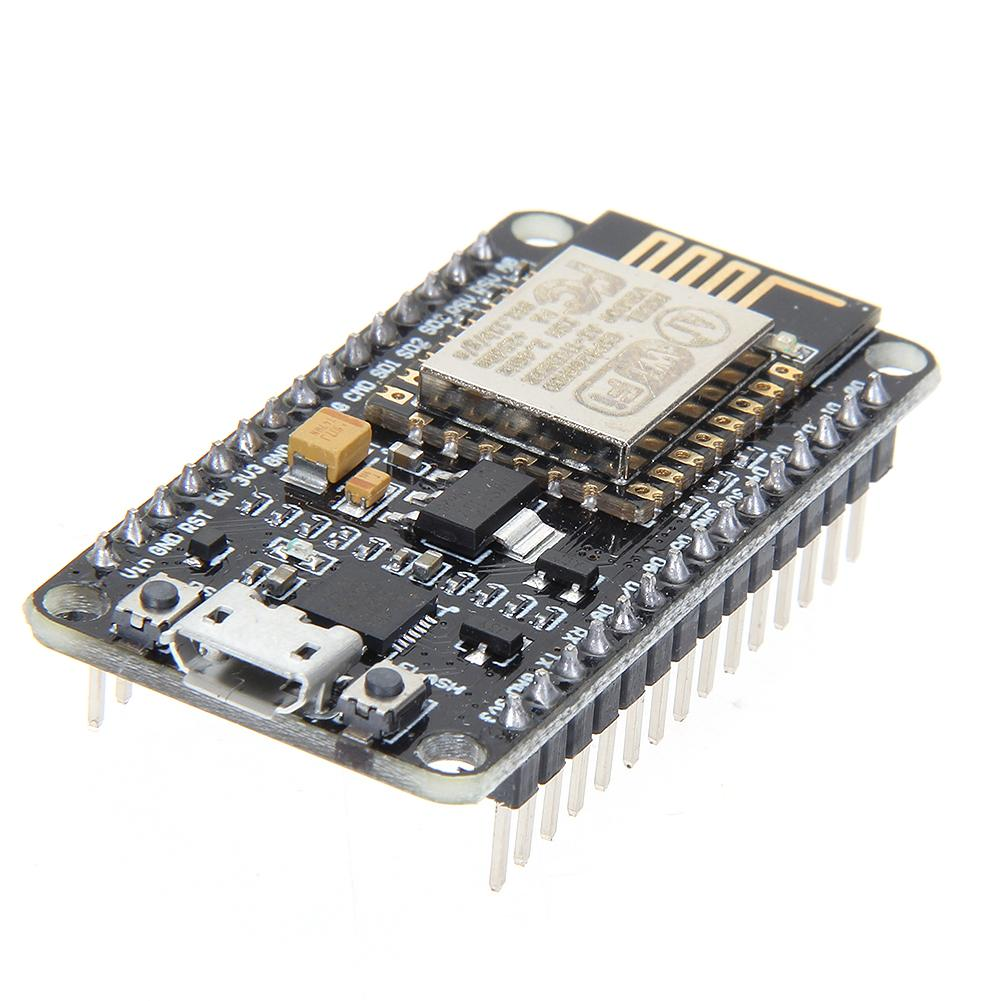
\includegraphics[scale=.1]{esp8266}
	\caption*{\footnotesize{Quelle: \mycite{esp8266}}}
	\label{fig:esp8266}
\end{wrapfigure}

\autoref{fig:esp8266} zeigt einen ESP8266 WLAN Mikrocomputer.
In Kombination mit einem Netzteil und Sensoren für Temperatur, Licht und Bewegung kann so eine \ac{DIY}-Wetterstation für weniger als zehn Euro gebaut werden.\myfootcite[Vgl.][]{bruhautomation_esp_sensor}

Der offene Quelltext von Home Assistant ermöglicht zudem, dass jederzeit nachvollzogen werden kann, was mit den eigenen Daten passiert.
Außerdem funktioniert Home Assistant vollständig offline.
Bei einem Internetausfall bleibt das Smart Home also weiter nutzbar.
Gleichzeitig bedeutet das auch, dass Dritte sich erst Zugriff zum eigenen Heimnetzwerk verschaffen müssen, damit ein Versuch unternommen werden kann Daten zu kompromittieren.

Zusammenfassend bietet Home Assistant Privatsphäre, Unabhängigkeit gegenüber des Internets, sowie eine hohe Bandbreite an verfügbaren Geräten und nutzbaren Schnittstellen.

\subsubsection{Nachteile}

Home Assistant wird von einer \glqq worldwide community of tinkerers and DIY enthusiasts.\grqq{}\myfootcite{hass_github_organization} entwickelt.
Gleichermaßen richtet sich Home Assistant als Produkt auch an Bastler und Tüftler.
So müssen Englischkenntnisse und Erfahrung im Umgang mit Linux und Computernetzwerken für die Einrichtung von Home Assistant vorhanden sein.\myfootcite[Vgl.][]{hass_getting_started}

Zudem befindet sich Home Assistant noch in aktiver Entwicklung und so fordern manche Änderungen der Software aktive Maßnahmen des Benutzers, wie etwa das Aktualisieren einer Konfigurationsdatei.\myfootcite[Vgl.][]{hass_breaking_change_example}

Home Assistant kann im jetzigen Zustand nur von technisch Versierten genutzt werden.

\subsection{Integrierte Lösung} % change title to actual product

% ein system, welches beim bau eines haus integriert wird.
% also ein gesamtsystem aus einer hand von einem unternehmen.

\subsubsection{Vorteile}

\subsubsection{Nachteile}

\subsection{Risiken}

% if used in combination with IoT: data breaches and loss of control
% power loss = no function
% smart home device with security flaw can be used to break into the local network

\subsection{Geschichte}

% idk -> wikipedia?

\subsection{Geschäftsmodelle}

% foreach:
% how does the business model work?
% example product?
% potential market?

\subsubsection{Geräte verkaufen} % TODO better title

% sell products like: philips lightning bulb

\subsubsection{Cloud Erweiterung} % TODO better title

% see: home assistant cloud by nabu casa

\subsubsection{Gesamtsystem} % TODO better title

% install a smart home integration in peoples homes who don't know how to do so themselves

\subsubsection{Alexa Skills} % TODO better title

% sell alexa skills
% create a skill with payment option

% https://developer.amazon.com/blogs/alexa/post/b8101123-f1b9-494c-8bbb-53e3850a1123/in-skill-purchasing-offers-jeff-bolton-s-voice-business-a-new-level-of-monetization

\section{Fazit}

% trends --> closed source, iot :/, automations! :D
% best business models
% home assistant empfehlung :)